\documentclass[12pt, letterpaper, oneside]{article}
%\documentclass[a4paper, 12pt, oneside]{ncc}
\usepackage{mathtext}          % русские буквы в формулах (с предупреждением \usepackage[warn]{mathtext})
\usepackage[T2A]{fontenc}            % внутренняя кодировка  TeX
\usepackage[utf8x]{inputenc}         % кодовая страница документа
\usepackage[english, russian]{babel} % локализация и переносы
%\usepackage{indentfirst}   % русский стиль: отступ первого абзаца раздела
%\usepackage{misccorr}      % точка в номерах заголовков
\usepackage{cmap}          % русский поиск в pdf
\usepackage{graphicx}      % Работа с графикой \includegraphics{}
%\usepackage{psfrag}        % Замена тагов на eps картинкаx
\usepackage{caption}      % Работа с подписями для фигур, таблиц и пр.
%\usepackage{soul}          % Разряженный текст \so{} и подчеркивание \ul{}
%\usepackage{soulutf8}      % Поддержка UTF8 в soul
\usepackage{fancyhdr}      % Для работы с колонтитулами
	\fancyhead[L, R]{}
	\fancyhead[C]{Отчёт о лабораторной работе 4.4.2.}
\usepackage{multirow}      % Аналог multicolumn для строк
\usepackage{geometry}
\usepackage{wrapfig}       %обтекание текстом
\usepackage{array}
\usepackage{mathrsfs}
\usepackage{float} %точное расположение таблиц и рисунков [H]
\usepackage{physics}
\usepackage{gensymb} %degree symbol

\usepackage{tikz}
 \usetikzlibrary{decorations.pathmorphing}
 \usetikzlibrary{patterns}
\usepackage{pgfplots}
\usepackage[europeanresistors,americaninductors, americancurrents]{circuitikz}

\pgfplotsset{compat=1.8}

\geometry{a4paper,left=1cm,right=1cm, top=2cm,bottom=1.9cm}

\title{Измерение энергии активации.}

\begin{document}
\maketitle
\noindent\textbf{\underline{1.Аннотация.}}\\
В работе измеряются величины остаточной индукции магнитного поля $B_r$, коэрцитивной силы $H_c$, амплитуда магнитной индукции $B_s$ и напряжённости магнитного поля $H_s$ предельной петли гистерезиса для ферромагнитных образцов из трёх различных матеиалов: феррита, пермаллоя и кремнистого железа — тороидной формы. Для измерений используются фигуры лиссажу, получаемые при помои электронного осциллографа, подключённого к установке, возбуждающей колебания. Схему установки см. на рис. 1.\\
\begin{figure}[h]
\centering
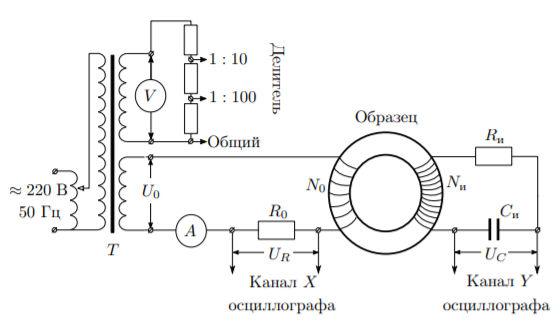
\includegraphics{scheme.png}
\caption{Схема экспирементальной установки.}
\end{figure}\\
\textbf{\underline{2.Теоретическое введение.}}\\
Для нахождения напряжённости поля в образце воспользуемся формулой, следующей из теоремы о циркуляции:
\begin{equation}\label{circ_H}
H = \frac{I N_0}{2\pi R},
\end{equation}
где $I$ — величина намагничивающего тока, $N_0$ — число витков в намагничивающей обмотке, а $R$ — средний радиус тора.\\
Намагничивающий ток измеряется при помощи ЭО с использоваинем закона Ома (см. рис. 1). Окончательно, исходя из \ref{circ_H}, получим
\begin{equation}\label{X_formula}
H = \frac{U_X N_0}{2\pi R R_0},
\end{equation}
Методика измерения магнитной индукции в образце основывается на формуле
\begin{equation}\label{Y_formula}
B = \frac{R_i C_i}{S N_i}U_{out},
\end{equation}
где $U_{out} = U_Y$ — выходное напряжение интегрирующей ячейки, $R_i$ и $C_i$ — её сопротивление и ёмкость соответственно, $S$ — площадь поперечного сечения образца, а $N_i$ — число витков в его вторичной обмотке.\\
Подключая $U_X$ и $U_Y$ к соответствующим каналам удаётся получить на экране осциллографа петлю гистерезиса. Для измеренияеё параметров используется сетка на экране.\\
Для калибровки масштаба шкал осциллографа в случае оси $X$ используется синусоидальный ток эффективное значение которого $I_{eff}$ измеряется независимо при помощи цифрового амперметра, пропускаемый через известное сопротивление $R_0$ (катушка образца на время калибровки закорачивалась). Рабочая формула в этом случае:
\begin{equation}\label{K_X_formula}
K_X = \frac{2R_0\sqrt{2}I_{eff}}{2x},
\end{equation}
где $K_X$ — масштаб по оси $X$, а $2x$ — длина горизонтального отрезка на экране.
В случае же оси $Y$ было произведено независимое (при помощи цифрового вольтметра и ЭО) измерение синусоидаль напряжения на клеммах "1/100" и "общий" делителя напряжений (см. рис. 1) (измерения также проводятся без подключения образца). Рабочая формула в этом случае:
\begin{equation}\label{K_Y_formula}
K_Y = \frac{2\sqrt{2}U_{eff}}{2y},
\end{equation}
где $K_Y$ — измеряемый масштаб, $U_{eff}$ — эффиктивное напряжение, измеряемое вольтметром, а $2y$ — длина вертикаьльного отрезка на экране осциллографа.\\
Для выяснения характерного времени разрядки конденсатора интегрирующей ячейки воспользуемся формулой $\tau_i = C_iR_i$. Параметры $C_i$ и $R_i$ указаны на установке. Подставляя их в формулу находим, что $\tau ≫ \frac{1}{\omega}$, где $\omega$ — частота напряжения, указанная на установке. Используемые значения: $R_i = 20\ кОм$, $C_i = 20\ мкФ$ $\omega = 50\ Гц$\\
\textbf{\underline{3.Приборы и материалы}}\\
Указанные на установке параметры представлены в таблице\\
\begin{table}[H]
\centering
\caption{Параметры измерительной установки, согласно маркировке}
\begin{tabular}{|c|c|c|}
\hline
$R_0,$ Ом & $R_i,$ кОм & $C_i,$ мкФ\\
\hline
0,22 & 20 & 20\\
\hline
\end{tabular}
\end{table}\noindent
В следующей таблице указаны параметры используемых образцов\\
\begin{table}[H]
\centering
\caption{Параметры используемых образцов, согласно маркировке}
\begin{tabular}{|c|c|c|c|c|}
\hline
Материал & $N_0,$ шт & $N_i,$ шт & $S,$ $см^2$ & $2\pi R,$ см\\
\hline
Феррит & 42 & 400 & 3,0 & 25\\
\hline
Пермаллой & 20 & 400 & 0,76 & 13,3\\
\hline
Кремнистое железо & 25 & 250 & 2,5 & 11\\
\hline
\end{tabular}
\end{table}
\noindent\textbf{\underline{4.Результаты измерений и обработка данных.}}\\
Полученные результаты измерений представлены ниже. Под $K_X$ и $K_Y$ понимается масштаб соответствующей оси осциллографа, согласно значениям на ручках прибора.
\begin{table}[H]\label{raw_data}
\centering
\caption{Измеренные значения напряжения}
\begin{tabular}{|m{2.1cm}|c|c||c|c||c|c||c|c|}
\hline
Материал & $h$, дел/5 & $K_Y$, $\frac{мВ}{дел}$ & $w$, дел/5 & $K_X$, $\frac{мВ}{дел}$ & $2X_c$, дел/5 & $K_X$, $\frac{мВ}{дел}$ & $Y_r$, дел/5 & $K_Y$, $\frac{мВ}{дел}$\\
\hline
Феррит & 40 & 20 & 37 & 200 & 30 & 10 & 31 & 10\\
\hline
Пермаллой & 20 & 50 & 10 & 50 & 46 & 10 & 18 & 50\\
\hline
Кремнистое железо & 25 & 50 & 36 & 200 & 32 & 20 & 24 & 20\\
\hline
\end{tabular}
\end{table}\noindent
В таблице ниже представлены значения, полученные при калибровке ЭО. Под $K_X$ и $K_Y$ понимается масштаб соответствующей оси осциллографа, согласно значениям на ручках прибора. $K_X^m$ и $K_Y^m$ — рассчитанный по измерениям масштаб соответствующих осей ЭО.
\begin{table}[H]
\centering
\caption{Проверка калибровки ЭО.}
\begin{tabular}{|c|c|c||c|c|c|}
\hline
$K_X$, $\frac{мВ}{дел}$ & $I_{eff}, мА$ & $K_X^m$, $\frac{мВ}{дел}$ & $K_Y$, $\frac{мВ}{дел}$ & $U_{eff}, мВ$ & $K_Y^m$, $\frac{мВ}{дел}$\\
\hline
10 & 152 & 9,45 & 10 & 27 & 9,54\\
\hline
20 & 306 & 19,05 & 20 & 55 & 19,44\\
\hline
50 & 765 & 47,60 & 50 & 136 & 48,08\\
\hline
200 & 1550 & 192,90 & — & — & —\\
\hline
\end{tabular}
\end{table}\noindent
Исходя из этих данных, можно заключить, что осциллограф откалиброван достаточно точно, чтобы использовать в расчётах величины $K_X$ и $K_Y$.\\
В таблице далее представлены рассчитанные по данным из таблицы 3 величины коэрцитивной силы ($H_c$), остаточной индукции ($B_r$) и амплитуд напряжённости ($H_s$) и индукции поля ($B_s$) для предельной петли гистерезиса каждого образца.\\
\begin{table}[H]
\centering
\caption{Измеренные характеристики различных образцов}
\begin{tabular}{|c|c|c|c|c|}
\hline
Материал & $H_c,$ $\frac{А}{м}$ & $B_r,$ Т & $H_s,$ $\frac{А}{м}$ & $B_s,$ Т\\
\hline
Феррит & 22,9 & 0,03 & 1221 & 0,16\\
\hline
Пермаллой & 31,4 & 1,56 & 136 & 1,73\\
\hline
Кремнистое железо & 66,1 & 0,12 & 1033 & 0,92\\
\hline
\end{tabular}
\end{table}\noindent
\textbf{\underline{5.Обсуждение результатов и выводы}}
\begin{Huge}
TODO: Вывод
\end{Huge}
\end{document}